%!TEX program = xelatex
%!TEX root = ./thesis.tex

\section{Experiment on the flat reinforcement learning solution to multi-modality tasks}
\subsection{Discussion on conventional flat reinforcement learning methods}
We observe contemporary end-to-end flat reinforcement learning methods fail to achieve good performance. We suggest that one of the important reason is the image features are much harder to learn than the state. The agent would tend to stuck at a local minimum when it has already learned the state features well, but has not been able to extract any useful information from the image. However, when the agent has finally learned the image features, the policy already converge to a relatively low-entropy distribution, and contemporary reinforcement learning methods cannot perform exploration again at this phase.

We take the task "movecont" as an example. In this task, a goal direction as sampled uniformly at random from the continuous range of angles: $[0,2\pi)$, at the beginning of each episode. The agent can only indicate the goal direction from the image, where there is a sphere object at the corresponding position.

A conventional method for encouraging exploration of reinforcement learning agents with continuous action space is entropy regularization. As we discussed in the section~\ref{sec_method_expadv_reg}, the entropy regularization method is not an effective method in the general case because it simply adds constant biases on the policy parameters and may dominate the learning of the original task.

An experiment on the effectiveness of entropy regularization is shown in Figure~\ref{rec_ent_reg}. The agents are trained using ACKTR algorithm with 32 parallel agents, minibatch-size 2560 and KL-divergence constraint 0.0003. The result shows that the agent easily fails to learn the original task when the weight on entropy term is too large. 

The change of average Standard Deviation of the policy distributions is shown in Figure~\ref{rec_std_ent_reg}. The agents' policy distributions appear to get stuck at certain level of standard deviation when the entropy term is not optimal.
\begin{figure}[!htbp]
	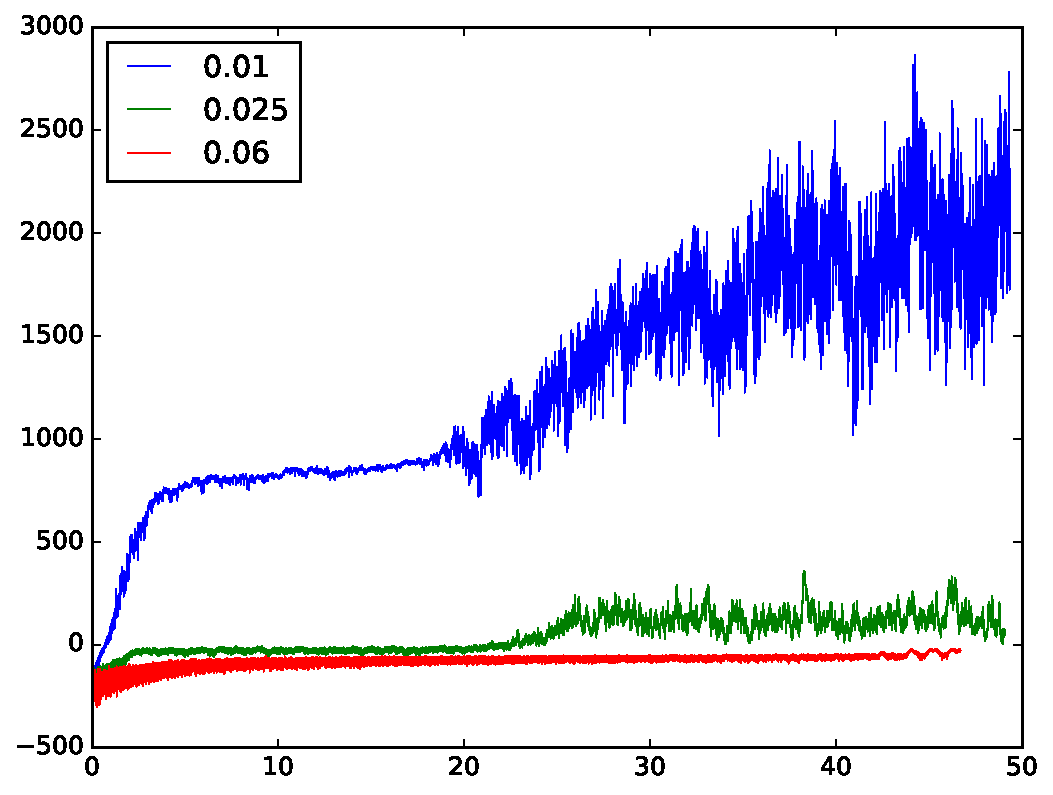
\includegraphics[width=\textwidth]{images/rec_ent_reg.pdf}
	\centering
	\caption{Performance of agents with different weight on entropy regularization term, the horizontal axis is the number of million timesteps and the vertical axis is the total episode reward averaged over the last 32 episodes}\label{rec_ent_reg}
\end{figure}

\begin{figure}[!htbp]
	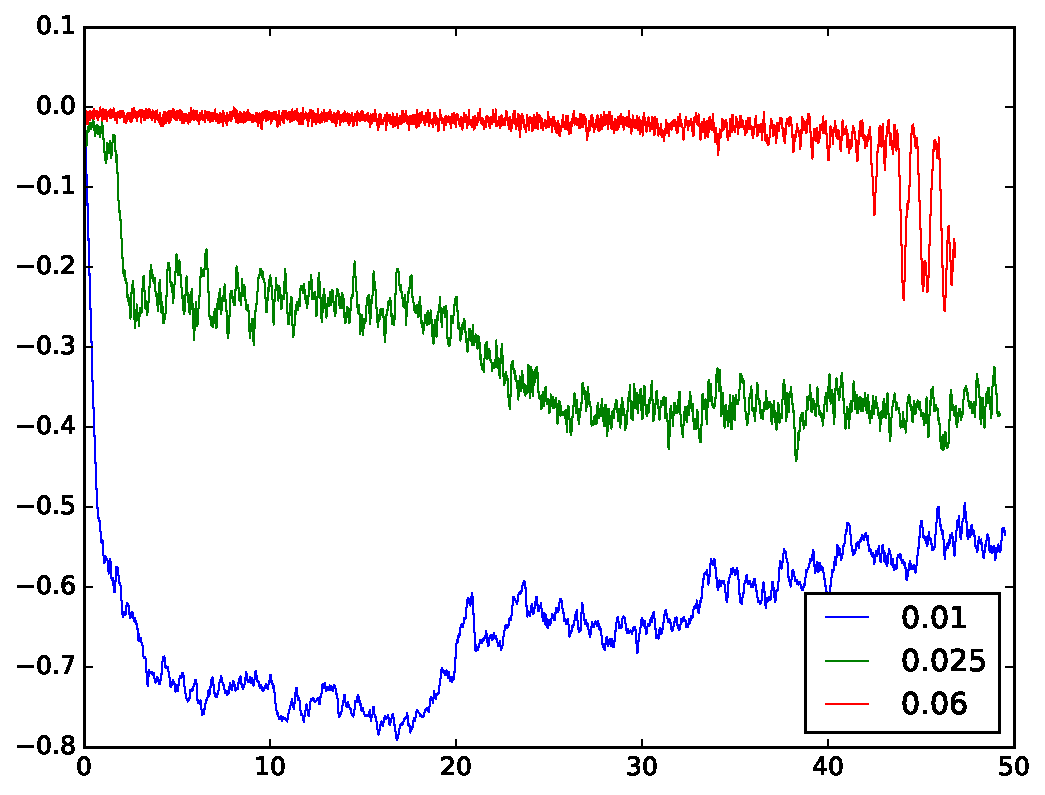
\includegraphics[width=\textwidth]{images/rec_std_ent_reg.pdf}
	\centering
	\caption{Logarithm of average standard deviation of the policy of agents in Figure~\ref{rec_ent_reg}, the horizontal axis is the number of million timesteps.}\label{rec_std_ent_reg}
\end{figure}

\subsection{Experiment on exceptional advantage regularization}
We discuss the effectiveness of exceptional advantage regularization method on multi-modality tasks in this section.

We first demonstrate the general patterns of the distribution on the advantage values on the simple multi-modality task "moveg2". In this task, the goal direction is sampled from 2 opposite directions. The task is much more simple than the "movecont" task because the agent only needs to learn from the image whether it needs to go forward or backward. 

The performance on the total return of an ACKTR agent is shown in Figure~\ref{rec_stat_moveg2}. The performance in terms of average reward per time-step is shown in Figure~\ref{rec_stat_moveg2_meanrt}, and the average standard deviation is shown in Figre~\ref{rec_stat_moveg2_std}.


\begin{figure}[!htbp]
	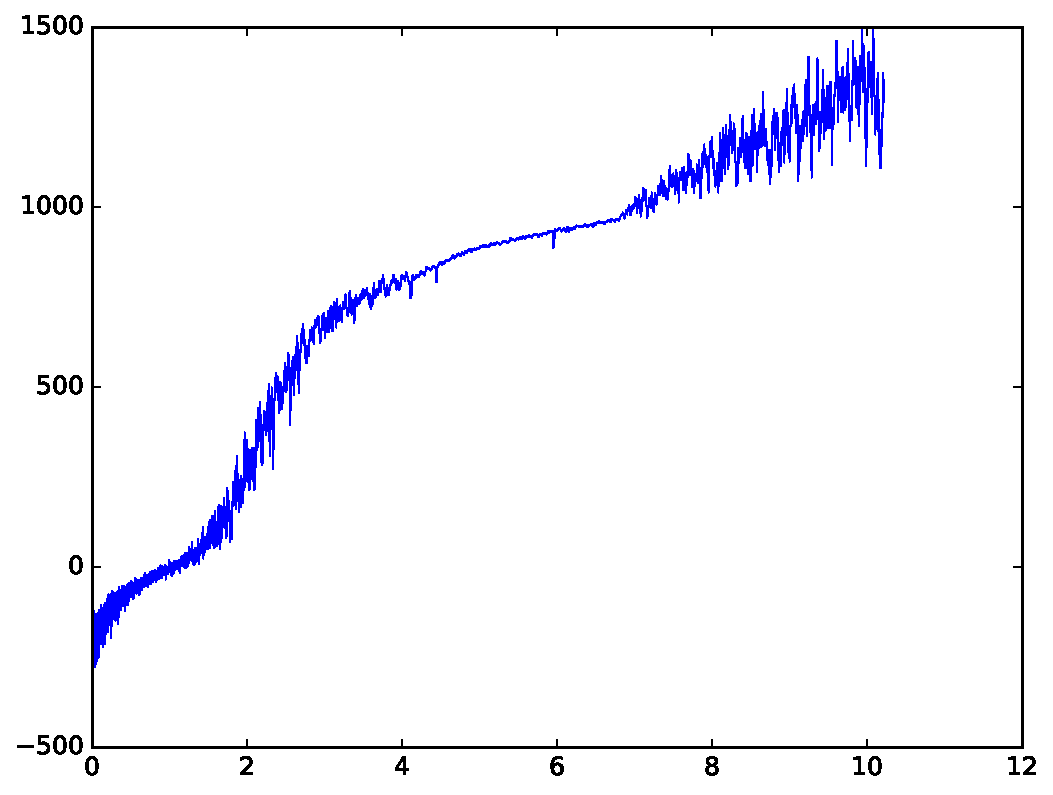
\includegraphics[width=0.7\textwidth]{images/rec_stat_moveg2.pdf}
	\centering
	\caption{Performance of ACKTR agent on the "moveg2" task, the horizontal axis is the number of million timesteps and the vertical axis is the total episode reward averaged over the last 20 episodes}\label{rec_stat_moveg2}
\end{figure}

\begin{figure}[!htbp]
	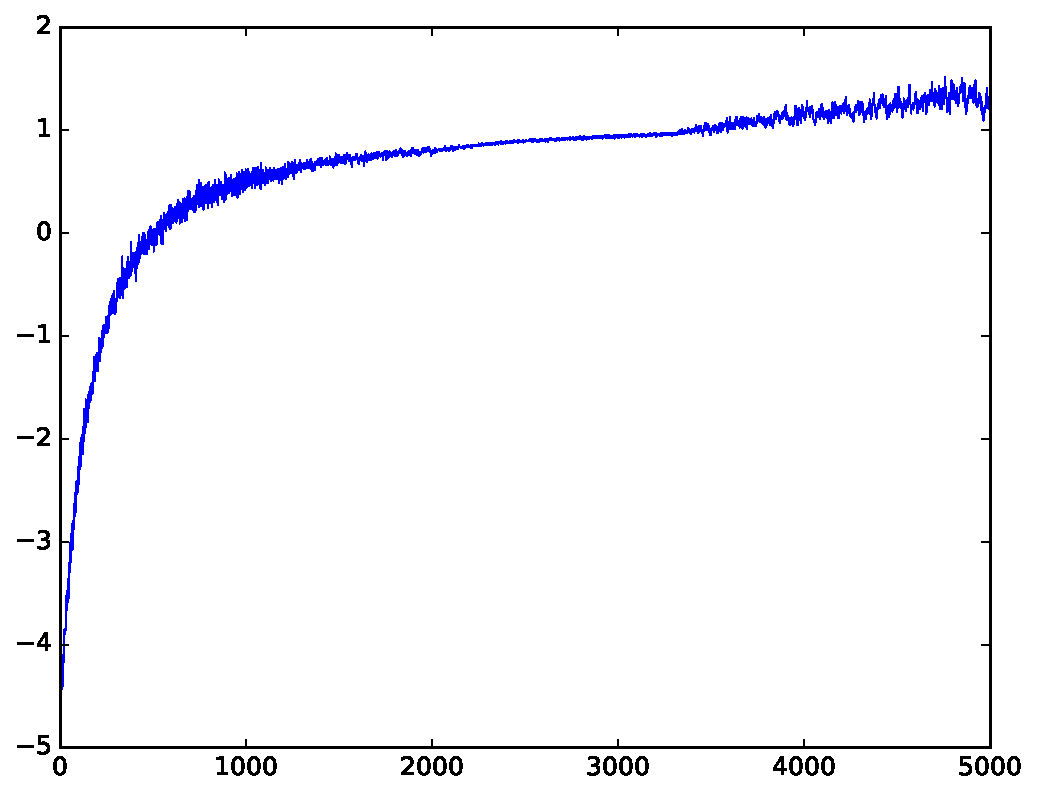
\includegraphics[width=0.7\textwidth]{images/rec_stat_moveg2_meanrt.pdf}
	\centering
	\caption{The avearge reward per time-step of ACKTR agent on the "moveg2" task, the horizontal axis is the number of training batches}\label{rec_stat_moveg2_meanrt}
\end{figure}

\begin{figure}[!htbp]
	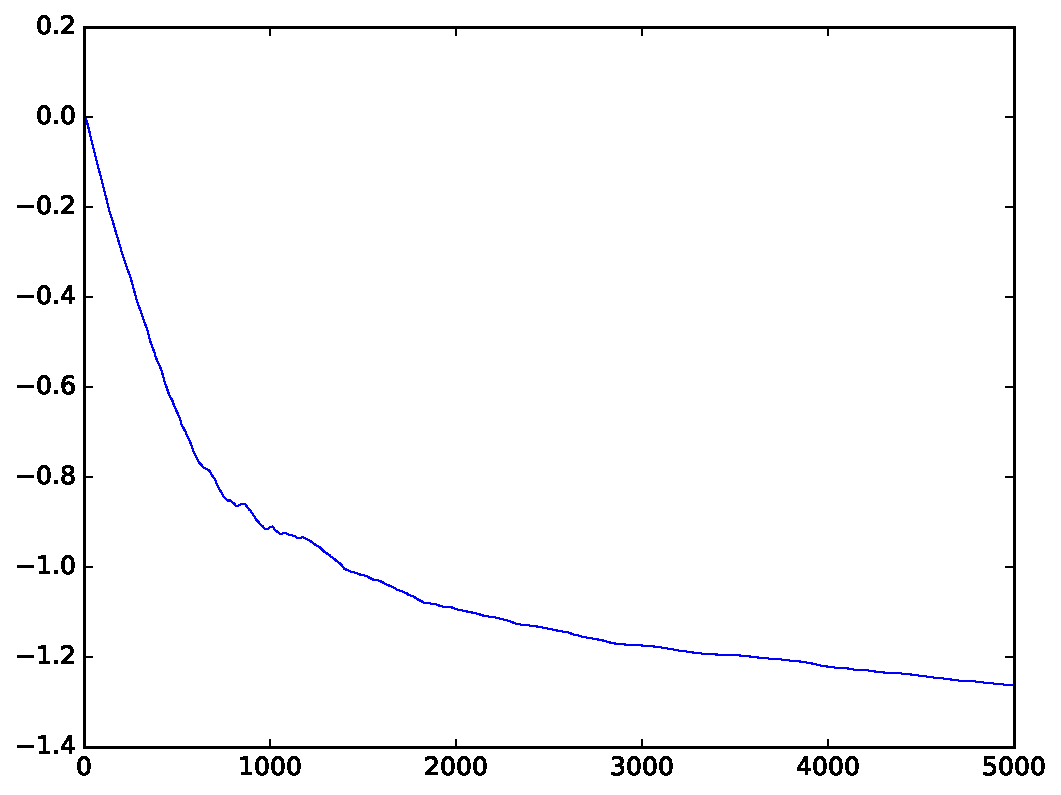
\includegraphics[width=0.7\textwidth]{images/rec_stat_moveg2_std.pdf}
	\centering
	\caption{The logarithm of avearge standard deviation of ACKTR agent's policy on the "moveg2" task, the horizontal axis is the number of training batches}\label{rec_stat_moveg2_std}
\end{figure}
The distribution of advantage values at the first batch (batch 0) is shown in Figure~\ref{vis_stats_0}. It can be seen that the advantage values are distributed uniformly across different values of log-likelihood because the critic model has not been trained. After the critic model has been trained for a reasonable amount of time, the marginal distribution advantage value tend to follow a normal distribution with zero mean. An example is shown in Figure~\ref{vis_stats_3000}, which is the distribution at batch 3000. However, the advantage values are likely to have higher values at low log-likelihood samples when the agent has just escaped from a local minimum. An example is Figure~\ref{vis_stats_4900}, which shows the the distribution of advantage values at batch 4900. It can be seen that the distribution becomes significantly different because many positive advantage points are spread across different log-likelihoods. 

Intuitively, a large number of points with low log-likelihood but high advantage value indicates that the agent needs to increase the degree of exploration. However, the figure~\ref{rec_stat_moveg2_std} on the change of standard deviation shows that the agent actually still keep decreasing the standard deviations of its policy even at this state. Therefore, the application of a exceptional advantage regularization term, could be useful in encouraging exploration in these cases.

\begin{figure}[!htbp]
	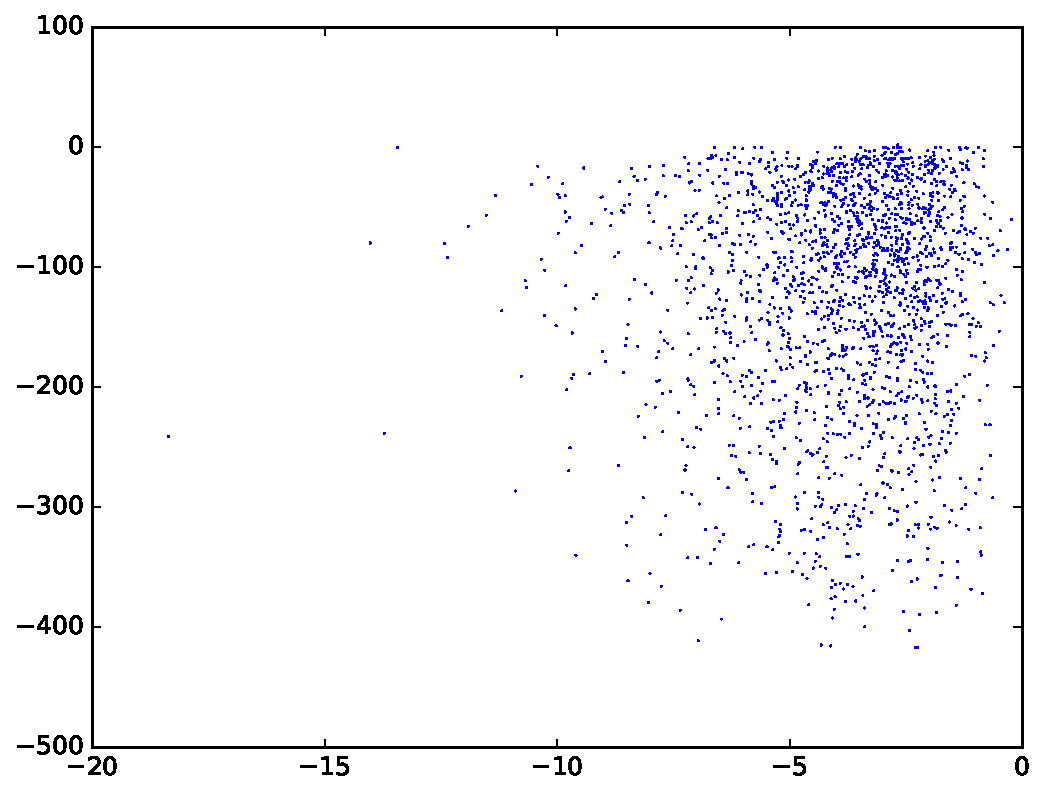
\includegraphics[width=\textwidth]{images/vis_stats_0.pdf}
	\centering
	\caption{The distribution of advantage values of the ACKTR agent at batch 0 on the "moveg2" task, the horizontal axis is the log-likelihood value}
	\label{vis_stats_0}
\end{figure}

\begin{figure}[!htbp]
	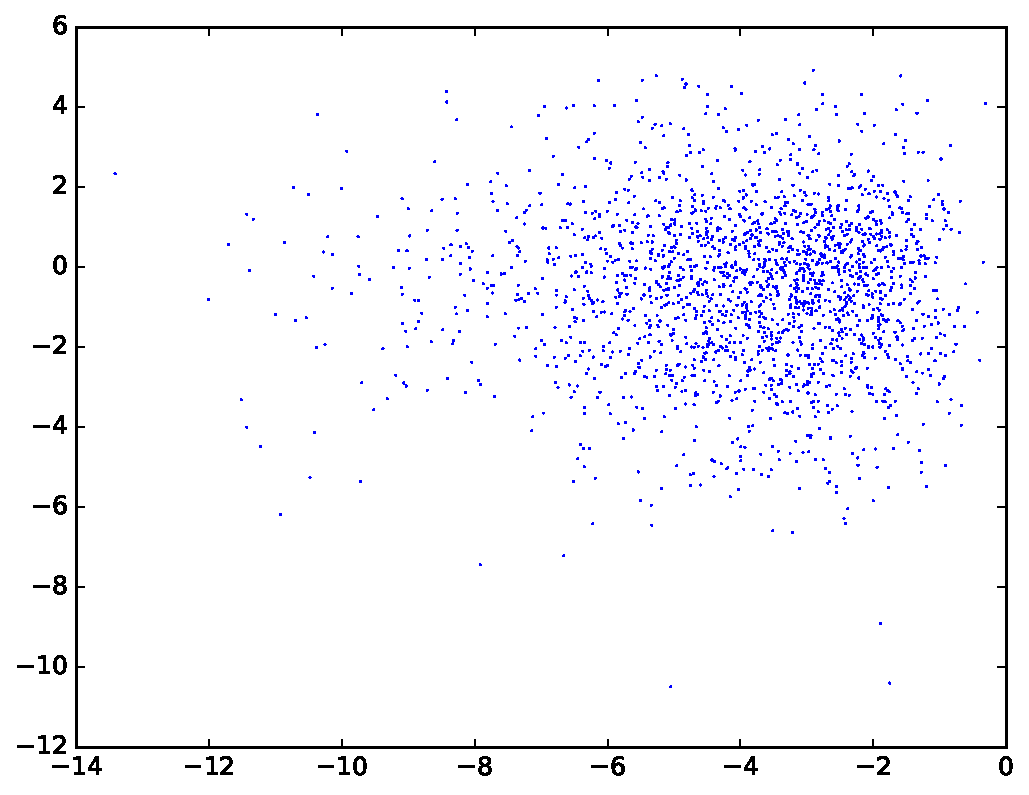
\includegraphics[width=\textwidth]{images/vis_stats_3000.pdf}
	\centering
	\caption{The distribution of advantage values of the ACKTR agent at batch 300 on the "moveg2" task, the horizontal axis is the log-likelihood value}
	\label{vis_stats_3000}
\end{figure}

\begin{figure}[!htbp]
	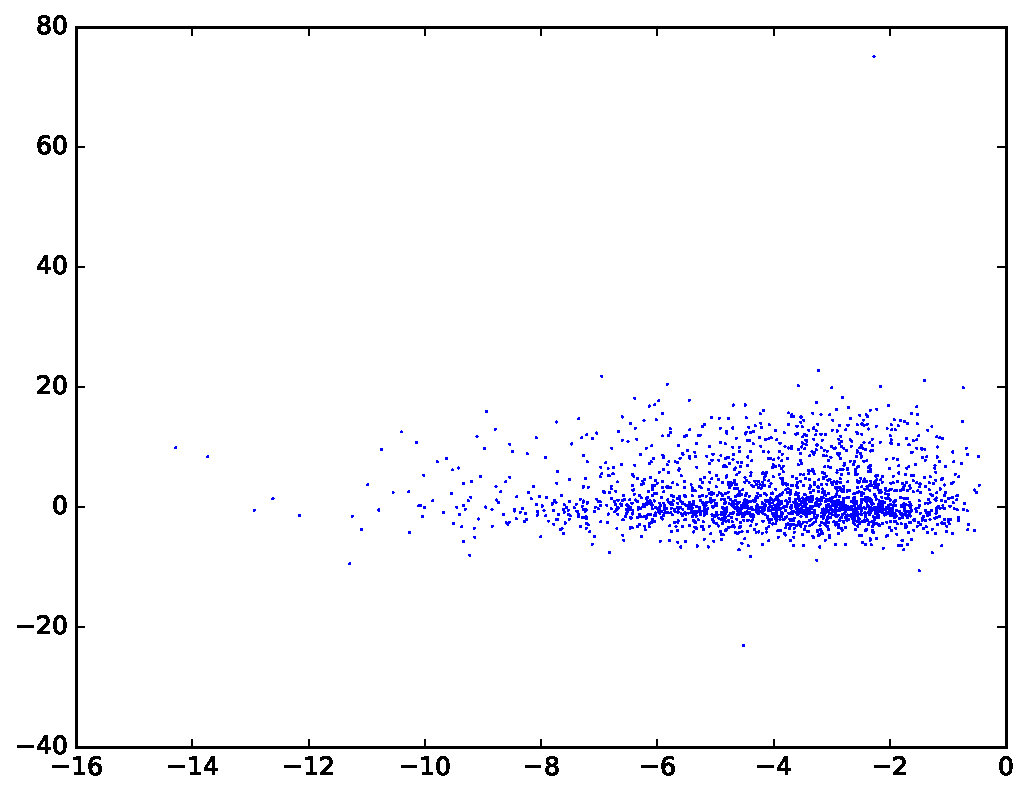
\includegraphics[width=\textwidth]{images/vis_stats_4900.pdf}
	\centering
	\caption{The distribution of advantage values of the ACKTR agent at batch 4900 on the "moveg2" task, the horizontal axis is the log-likelihood value}
	\label{vis_stats_4900}
\end{figure}

We then verify the performance of exceptional advantage regularization on the 'movecont' task.
The performance of an ACKTR agent with different weights exceptional advantage regularization on the in Figure~\ref{rec_adv_reg}, and the average standard deviation parameter of their policies are shown in Figure~\ref{rec_std_adv_reg}. All the agents are trained with batch-size 2560 and KL-divergence constraint 0.0003. The weight-0 agent is the same as the original ACKTR agent without any exploration regularization, and it could only achieve a total reward of around 2000 at the end of training. The agent with exceptional advantage regularization weight 0.04 can improve rapidly in the early phase before 40 million timestep, but gets stuck at around 3500. This shows that the exceptional advantage regularization method could have adverse effect on the convergence of policy in the late phase of training, which is also indicated in by average std curve. The agent with exceptional advantage regularization weight 0.01 achieves the best final performance. Its average standard deviation shows that the agent manages to increase its policy entropy and re-explore the environment after it has escaped from a local minimum.
\begin{figure}[!htbp]
	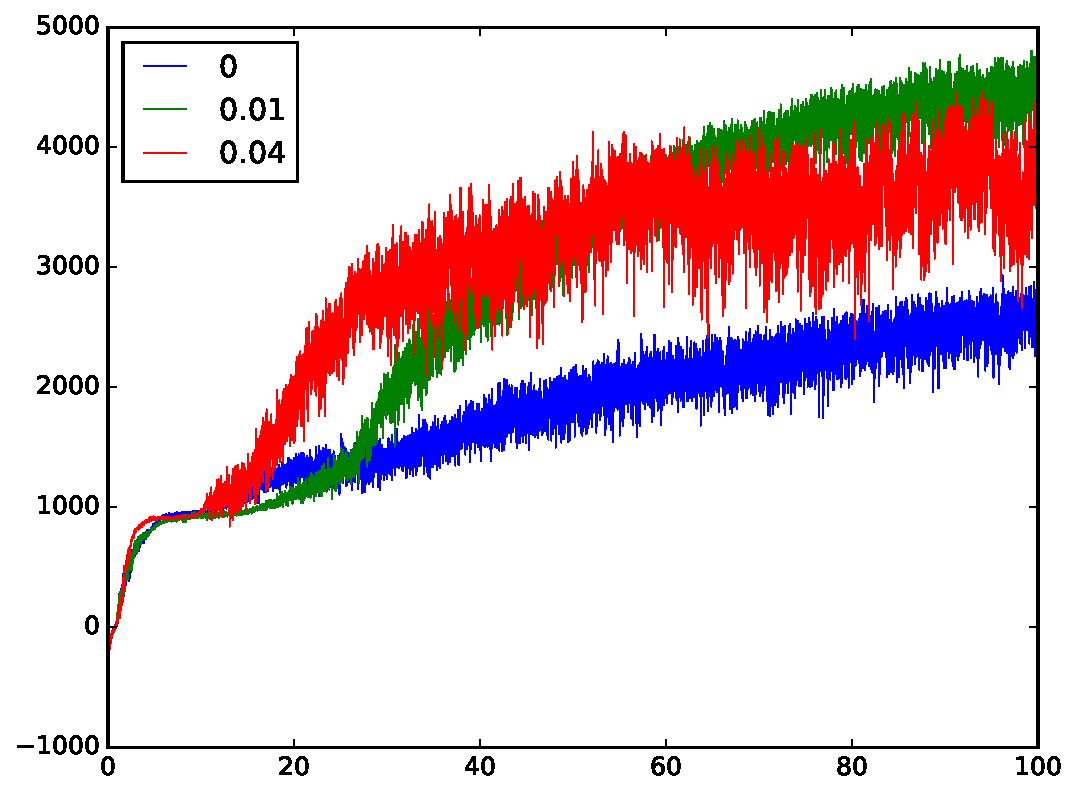
\includegraphics[width=\textwidth]{images/rec_adv_reg.pdf}
	\centering
	\caption{Performance of agents with different exceptional advantage regularization weights, the x-axis is the number of million time-steps and the y-axis is the total episode reward averaged over the last 32 episodes}\label{rec_adv_reg}
\end{figure}

\begin{figure}[!htbp]
	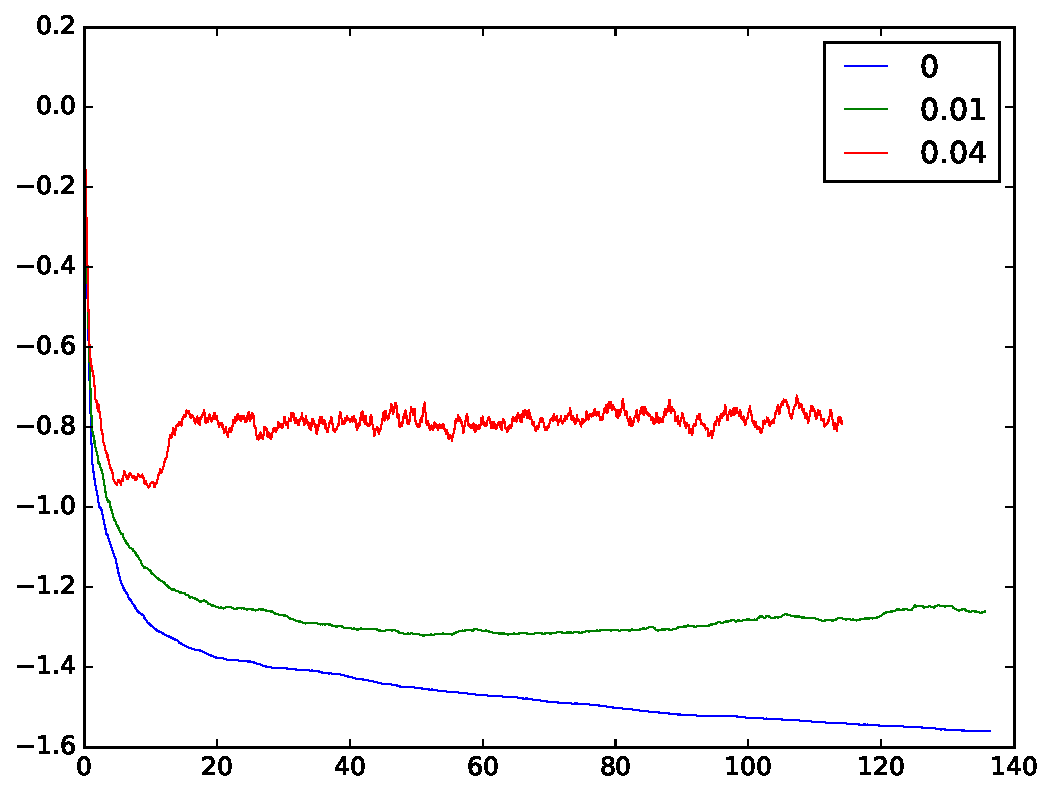
\includegraphics[width=\textwidth]{images/rec_std_adv_reg.pdf}
	\centering
	\caption{The logarithm of avearge standard deviation of agents with different exceptional advantage regularization weights, the horizontal axis is the number of million time-steps and the vertical axis is the total episode reward averaged over the last 32 episodes}\label{rec_std_adv_reg}
\end{figure}

\subsection{Experiment on the Robust Concentric Mixture Gaussian Policy}
The effectiveness of robust concentric mixture Gaussian policy agent in exploration of task "movecont" is verified in this section. 

The performance of an ACKTR mixture Gaussian policy agent is shown in Figure~\ref{rec_mix}. The results shows that the mixture Gaussian policy agents have slower learning rates compared to pure Gaussian policy agents. However, the agents are able to achieve a good final performance, with a total reward of around 4000 when the KL-divergence is set properly.

\begin{figure}[!htbp]
	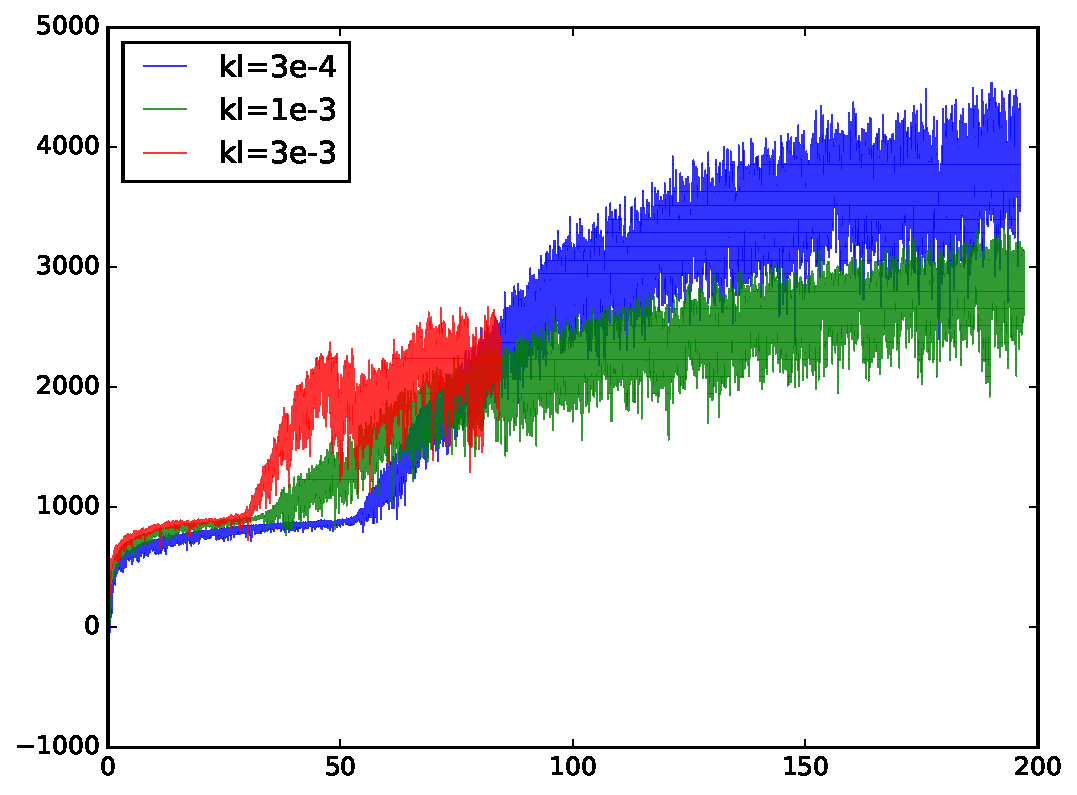
\includegraphics[width=\textwidth]{images/rec_mix.pdf}
	\centering
	\caption{Performance of ACKTR agents with different KL-divergence constraints, the x-axis is the number of million time-steps and the y-axis is the total episode reward averaged over the last 32 episodes}\label{rec_mix}
\end{figure}
